% Opisanie tego jak zbudowane jest UI ogólnie, nawiązanie, że opisane zostaną tylko te najważniejsze
Całość kodu źródłowego aplikacji, która odpowiedzialna jest za renderowanie interfejsu użytkownika
wykorzystuje paradygmat programowania komponentowego -- pozwala na projektowanie, implementację oraz
testowanie elementów aplikacji niezależnie od siebie. Dodatkowo, jeżeli zaistnieje taka potrzeba,
część kodu źródłowego może być stworzona~w~zupełnie innym języku programowania, a~następnie
dołączona do aplikacji, gdzie będzie idealnie współpracować~z~resztą obecnych już komponentów
\cite{component-programming}. Interfejs użytkownika~w~aplikacji jest~w~języku angielskim. Został
stworzony~w~taki sposób, aby finalna aplikacja mogła być wykorzystywana przez użytkowników nie
tylko~z~Polski.

% Opis poszególnych, ważnych składowych UI ze snippetami
\subsection{Elementy interfejsu}
Głównymi elementami interfejsu są komponenty odpowiedzialne za:
\begin{itemize}
  \item[--] konfigurację sensora dla danego laboratorium,
  \item[--] wyświetlanie zadań do wykonania oraz wygenerowanych danych,
  \item[--] przyjmowanie oraz weryfikowanie odpowiedzi wpisywanych przez użytkownika,
  \item[--] prezentowanie wzorów oraz danych niezbędnych do obliczeń,
  \item[--] wyświetlanie wygenerowanego wykresu.
\end{itemize}
Powyższe elementy przedstawione zostały na rysunkach \ref{img:config-tasks},
\ref{img:generated-graph}, \ref{img:theory}.

\begingroup
\begin{figure}[!htbp]
  \centering
  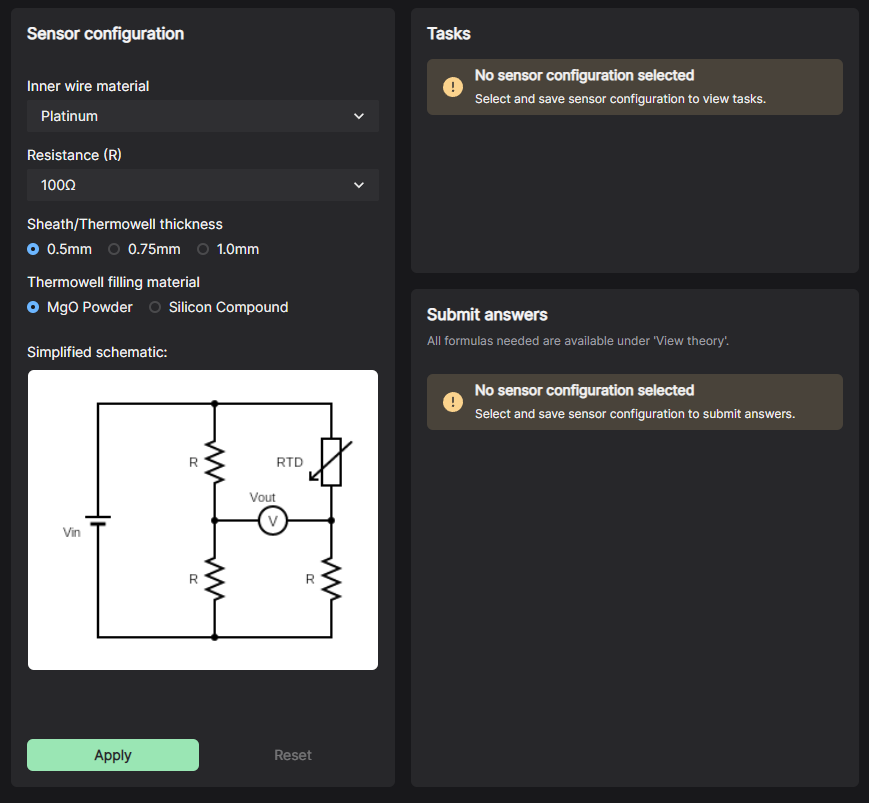
\includegraphics[width=0.65\textwidth]{app-ui/config-tasks}
  \caption{\label{img:config-tasks}Komponenty do konfiguracji, wyświetlania zadań~i~przyjmowania
    odpowiedzi.}
\end{figure}

\begin{figure}[!htbp]
  \centering
  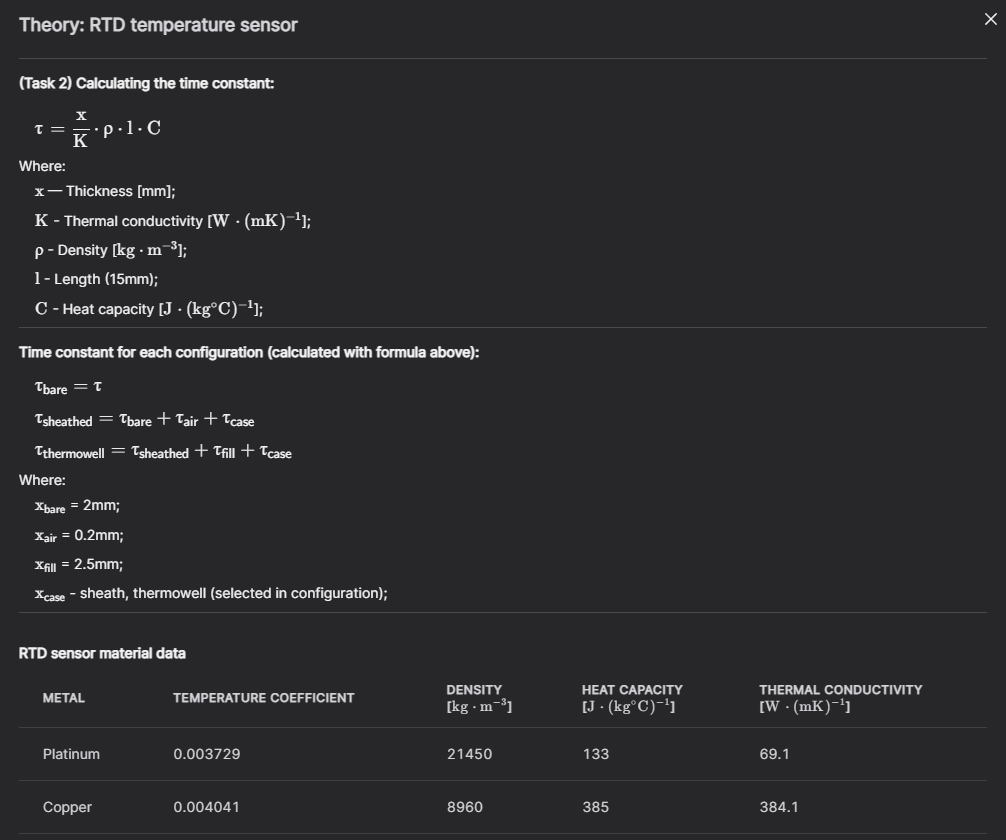
\includegraphics[width=0.65\textwidth]{app-ui/theory}
  \caption{\label{img:theory}Komponent prezentujący wzory oraz dane.}
\end{figure}

\begin{figure}[!htbp]
  \centering
  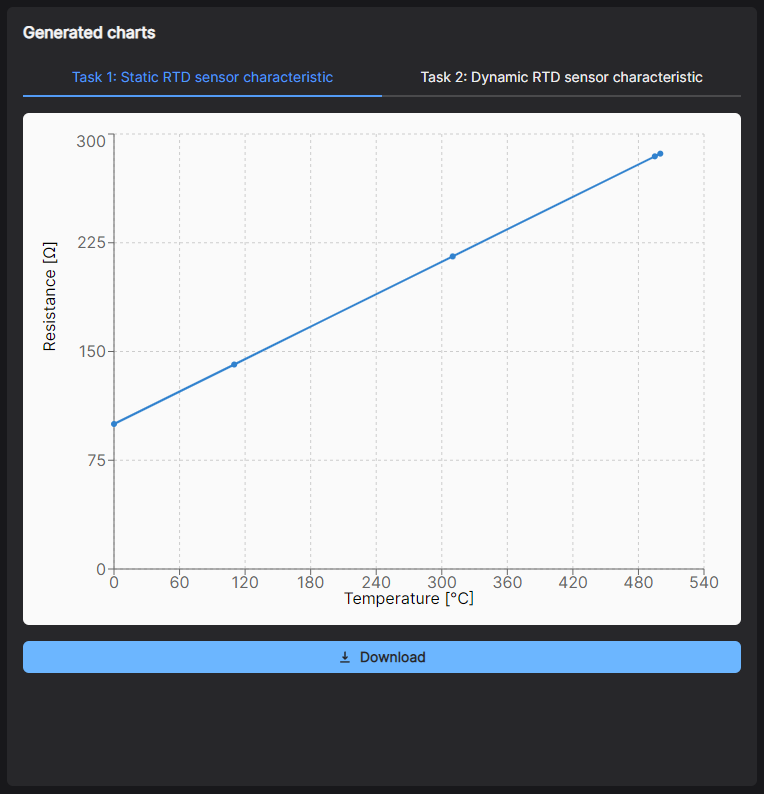
\includegraphics[width=0.65\textwidth]{app-ui/generated-graph}
  \caption{\label{img:generated-graph}Komponent wyświetlający wygenerowany wykres.}
\end{figure}
\endgroup

\subsubsection{Komponent do konfiguracji sensorów}
Dla każdego sensora możliwa jest zmiana jego parametrów. Do implementacji wykorzystana została
metoda dynamicznego mapowania pól~w~całym komponencie na podstawie pliku konfiguracyjnego,
odpowiadający za to kod przedstawiony został na rysunku \ref{lst:config-field-map}. Dane pole
posiada dwa różne warianty do wyboru -- wybór~z~listy (wykorzystywany~w~przypadkach, gdy dany
parametr ma więcej opcji do wyboru) lub przycisk typu radio (dla przypadków, gdzie opcji do wyboru
jest nie więcej jak trzy). Na rysunku \ref{lst:config-field} przedstawiony został kod, który
renderuje pojedyncze pole na podstawie informacji zawartych~w~pliku konfiguracyjnego, którego
fragment przedstawiony został na rysunku \ref{lst:config-field-data}.

\addimage{0.9}{code/config-field-map}{\label{lst:config-field-map}Funkcja dynamicznie mapująca pola
  na podstawie pliku konfiguracyjnego}

\addimage{0.9}{code/config-field}{\label{lst:config-field}Kod komponentu pojedynczego pola
  konfiguracyjnego}

\addimage{0.9}{code/config-field-data}{\label{lst:config-field-data}Fragment pliku zawierającego
  dane do generowania pól konfiguracyjnych}

Plik konfiguracyjny ma formę tablicy zawierającej obiekty, które definują dane pole. Każdy obiekt
składa się~z~par klucz-wartość. Klucz \colortt{sensor} określa do jakiego laboratorium przynależą
definiowane wartości, \colortt{id} wykorzystywany jest przy manipulowaniu stanem, którego zadaniem
jest przechowywanie informacji~o~obecnej konfiguracji sensora, natomiast \colortt{type} pozwala na
zdefiniowanie jaki wariant pola konfiguracyjnego ma zostać wyświetlony. Zarządzanie stanem oraz jak
zostało to rozwiązane~w~aplikacji opisane zostało~w~rozdziale \ref{sect:context}. Pozostałe klucze
-- \colortt{label, options, optionLabels, defaultValue} wykorzystywane są do określenia
wyświetlanego tytułu pola konfiguracyjnego, opcji dostępnych do wyboru oraz domyślnie
wybranej opcji.

\subsubsection{Komponent wyświetlający zadania oraz wygenerowany zestaw danych}
\lipsum[1]


\subsubsection{Komponent odpowiedzialny za przyjmowanie i weryfikację odpowiedzi}
\lipsum[1]


\subsubsection{Komponent prezentujący wzory oraz dane niezbędne do obliczeń}
Część teoretyczna do każdego laboratorium prezentowana jest~w~postaci okna dialogowego. Taka
implementacja została wykorzystana, aby użytkownik nie musiał zamykać strony~z~wykonywanym
ćwiczeniem (co skutkowałoby utratą postępów, ponieważ aplikacja nie posiada bazy danych). Zawartość
okna dialogowego konfigurowana jest przez dwa dodatkowe komponenty -- \texttt{Formula, Table},
których zadaniem jest generowanie odpowiednio listy wzorów oraz tabel~z~danymi na podstawie plików
konfiguracyjnych. Kod źródłowy odpowiadający za generowanie listy wzorów oraz tabel przedstawiony
jest~w~listingach \ref{lst:theory-formula} oraz \ref{lst:theory-table}, natomiast~w~listingach
\ref{lst:formula-config}, \ref{lst:table-config} przedstawione zostały fragmenty plików, które
zawierają informacje jakie wzory oraz tabele mają zostać wygenerowane przez komponenty.

\addsnippet{0.9}{code/theory-formula}{\label{lst:theory-formula}Kod komponentu odpowiedzialnego za
  generowanie listy wzorów}

\addsnippet{0.9}{code/theory-table}{\label{lst:theory-table}Komponent generujący tabele~z~danymi do
  ćwiczenia~w~oknie dialogowym}

\addsnippet{0.9}{code/formula-config}{\label{lst:formula-config}Fragment pliku~z~informacjami o
  wzorach do wyświetlenia~w~oknie dialogowym}

\addsnippet{0.9}{code/table-config}{\label{lst:table-config}Fragment pliku konfiguracyjnego do
  komponentu~z~tabelami}

Ponieważ pliki konfiguracyjne mają format tablicy~z~obiektami, to generowanie kolejnych wzorów oraz
wierszy tabeli wykonywane jest przez mapowanie kolejnych wartości. Odpowiednie miejsca~w~kodzie,
gdzie wstawione są nazwy zmiennych odczytujących klucze~z~konfiguracji, uzupełniane są pobranymi
informacjami.


\subsubsection{Komponent wyświetlający wygenerowany wykres}
Generowanie wykresów~w~aplikacji wykorzystuje do tego bibliotekę \textit{Recharts}. Udostępnia ona
komponenty \texttt{LineChart, CartesianGrid, XAxis, YAxis, Line}, które połączone pozwalają na
wyświetlanie wykresów. Dane, które mają być wykreślone podawane są poprzez zewnętrzne atrybuty,
ponieważ generowane są~w~komponencie danego laboratorium (implementacja przedstawiona
została~w~rozdziale \ref{sect:laboratory}).

Dodatkowo wykorzystana została biblioteka \textit{recharts-to-png}, która pozwala na zapisywanie
wykresów jako obrazów~w~formacie PNG, aby można było je~w~późniejszym czasie wykorzystać,
przykładowo pisząc sprawozdanie~z~wykonanego ćwiczenia laboratoryjnego. Implementacja tej
funkcjonalności przedstawiona została~w~listingu \ref{lst:chart-download}.

\addsnippet{0.9}{code/chart-download}{\label{lst:chart-download}Implementacja funkcjonalności
  zapisywania wykresów jako obrazy}

Aplikacja posiada dwa warianty komponetu do wyświetlania wykresu -- \texttt{SingleLineChart} oraz
\texttt{MultiLineChart}. Wykorzystywane są odpowiednio, tam gdzie potrzebny jest wykres, który
posiada tylko jedną linię lub który posiada wiele linii (w przypadku aplikacji jest to
laboratorium~z~sensorami temperatury, gdzie wykresy do charakterystyk dynamicznych posiadają trzy
linie).

